%%%%%%%%%%%%%%%%%%%%%%%%%%%%%%%%%%%%%%%%%%%%%%%%%%%%%
%% File: main.tex
%% Authors: Petros Chanas, Konstantinos Vasilopoulos
%% Last update: April, 2022
%% Description: Provides our assignment 
%% regarding Open Source Software Quality Testing
%%and parameters of rating the performance and quality
%%of software developed of open source applications
%%%%%%%%%%%%%%%%%%%AUEB2021-2022%%%%%%%%%%%%%%%%%%%%%
%% Character encoding: UTF-8
%%%%%%%%%%%%%%%%%%%%%%%%%%%%%%%%%%%%%%%%%%%%%%%%%%%%%


\documentclass[a4paper, 11pt]{article}
\usepackage[margin=1in]{geometry}
% Set the font (output) encoding
\usepackage[LGR]{fontenc}
\usepackage{pdfpages}
% Greek-specific commands
\usepackage[greek]{babel}
\usepackage{graphicx}
\usepackage[T1]{fontenc}
\usepackage{tgtermes}
%\usepackage{background}
\graphicspath{ {./images/} }
%\thispagestyle{empty}
%\backgroundsetup{
%scale=1,
%angle=0,
%opacity=.1,  %% adjust
%contents={
\includegraphics[width=\paperwidth,height=\paperheight]{images/sourceCode.jpg}}
%}
%
\includegraphics[width=\paperwidth, height=\paperwidth]{images/universe.jpg}}
\title{\textbf{\textlatin{ Open source software quality}}}
\author{{\textit{Κωνσταντίνος Βασιλόπουλος\(\bullet\)3180018}\\*\textit{Πέτρος Χάνας\(\bullet\)3170173}}\\*
\includegraphics[width=4cm, height=3cm]{oSource}}
\date{\today}
\begin{document}
\includepdf{assets/ekswfyllo.pdf}
\maketitle

{\fontfamily{cmss}\selectfont
\begin{abstract}
Σε αυτήν την εργασία θα αναφερθούμε στους τρόπους ανάπυτηξης ελεύθερου λογισμικού
και στα ενδεχόμενα προβλήματα τα οποία προκύπτουν ως προς τον προγραμματισμό και το 
\textlatin{debugging} αυτού καθ'όλη τη διάρκεια ζωής του. Επίσης θα μελετήσουμε τους 
τρόπους αξιολόγησης του λογισμικού από τρίτους παράγοντες όπως εταιρείες, δημόσιοι οργανισμοί 
αλλά και από τους ίδιους τους χρήστες. Ουσιαστικα, η ποιότητα του ανοιχτού-ελεύθεροου λογισμικού 
συνίσταται από κάποιους βασικούς πυλώνες άμεσα εξαρτώμενος από το ίδιο το λογισμικό όπως η ταχύτητά
του, η αξιοπιστία του, η ευκολία στην χρήση του αλλά και την περιήγησή του και πολλά άλλα. Εν ολίγοις, 
θα αναλύσουμε όλες τις πτυχές ανάπτυξης και αξιολόγησης της ποιότητας λογισμικού ανοιχτού κώδικα 
διανθίζοντας όλα τα επιμέρους στοιχεία που συγκροτούν αλλά και καθιστούν το λογισμικό έτοιμο προς διάθεση 
στο ευρύ κοινό.
\end{abstract}

{\fontfamily{cmss}\selectfont\section{Τι είναι το λογισμικό ανοιχτού κώδικα\textlatin{;}}}
%%perigrafh open source code by definition
%%famous examples etc.
 Συχνά θα ακούσουμε ανθρώπους της πληροφορικής να αναφέρονται σε συγκεκριμένα προγράμματα ως «ανοιχτού κώδικα» ή «ελεύθερου λογισμικού». Εάν ένα πρόγραμμα είναι ανοιχτού κώδικα, ο πηγαίος κώδικας του είναι ελεύθερος διαθέσιμος στους χρήστες του. Οι χρήστες του - και οποιοσδήποτε άλλος - έχουν τη δυνατότητα να λάβουν αυτόν τον πηγαίο κώδικα, να τον τροποποιήσουν και να διανείμουν τις δικές τους εκδόσεις του προγράμματος. Οι χρήστες έχουν επίσης τη δυνατότητα να διανέμουν όσα αντίγραφα του αρχικού προγράμματος θέλουν. Οποιοσδήποτε μπορεί να χρησιμοποιήσει το πρόγραμμα για οποιονδήποτε σκοπό. δεν υπάρχουν χρεώσεις αδειοδότησης ή άλλοι περιορισμοί στο λογισμικό. Για παράδειγμα, το \textlatin{Ubuntu Linux} είναι ένα λειτουργικό σύστημα ανοιχτού κώδικα. Μπορείτε να κατεβάσετε το \textlatin{Ubuntu}, να δημιουργήσετε όσα αντίγραφα θέλετε και να τα δώσετε στους φίλους σας. Μπορείτε να εγκαταστήσετε το Ubuntu σε απεριόριστο αριθμό υπολογιστών. Μπορείτε να δημιουργήσετε αντίγραφα του δίσκου εγκατάστασης του \textlatin{Ubuntu} και να τα διανείμετε. Εάν είχατε ιδιαίτερα κίνητρα, θα μπορούσατε να κατεβάσετε τον πηγαίο κώδικα για ένα πρόγραμμα στο Ubuntu και να το τροποποιήσετε, δημιουργώντας τη δική σας προσαρμοσμένη έκδοση αυτού του προγράμματος - ή του ίδιου του \textlatin{Ubuntu}. Όλες οι άδειες ανοιχτού κώδικα σάς επιτρέπουν να το κάνετε αυτό, ενώ οι άδειες κλειστού κώδικα επιβάλλουν περιορισμούς σε εσάς.\\*
\\*
\section{Ιστορική Αναδρομή}
Κατά τη διάρκεια των πρώτων δεκαετιών της πληροφορικής, ήταν ο κανόνας και όχι η εξαίρεση η κοινή χρήση αναγνώσιμου πηγαίου κώδικα από τον άνθρωπο. Στις δεκαετίες του 1950 και του 1960 σχεδόν όλο το λογισμικό που παρήχθη από ακαδημαϊκούς και εταιρικά ερευνητικά εργαστήρια, όπως τα \textlatin{Bell Labs} της  \textlatin{AT&T}, εργάστηκαν σε συνεργασία. Όλοι είχαν μακροχρόνιες παραδόσεις ανοιχτού χαρακτήρα και συνεργασίας, άτυπες για τον ακαδημαϊκό χώρο, και ως εκ τούτου, ακόμη κι αν το λογισμικό δεν ήταν επίσημα διαθέσιμο στο κοινό, ο πηγαίος κώδικας τους ήταν ευρέως κοινός. Οι εταιρείες ηλεκτρονικών υπολογιστών διένειμαν επίσης τον πηγαίο κώδικα του λογισμικού που έστειλαν μαζί με το υλικό, για δύο λόγους. Πρώτον, δεν έβλεπαν το λογισμικό ως εμπόρευμα προς πώληση μέσω αδειοδότησης. Δεύτερον, οι χρήστες τροποποιούσαν συχνά οι ίδιοι το λογισμικό επειδή δεν θα λειτουργούσε σε διαφορετικό υλικό ή λειτουργικό σύστημα χωρίς κάποια παρέμβαση στον "κορμό" του, καθώς και για να διορθώσουν σφάλματα ή να προσθέσουν νέες λειτουργίες.

Το να έχουν διαθέσιμο τον πηγαίο κώδικα ήταν νευραλγικής σημασίας για τους κατασκευαστές, καθώς η δημιουργία διαφορετικών \textlatin{binary files} (ή μεταγλωττισμένου κώδικα) για διαφορετικό υλικό δεν ήταν καθόλου πρακτική και 
συχνά δημιουργούσε μεγάλες επιπλοκές που οδηγοούσαν σε λογισμικό μή προσπελάσιμο λογισμικό, δλδ μη ικανό να περαιωθούν οι λειτουργίες του. Ορισμένα πανεπιστήμια είχαν ακόμη και μια πολιτική που απαιτούσε όλα τα λογισμικά που είναι εγκατεστημένα στους υπολογιστές στα εργαστήριά τους να συνοδεύονται από δημοσιευμένους πηγαίους κώδικες.

Το 1953, το τμήμα \textlatin{UNIVAC} του \textlatin{Remington Rand} ανέπτυξε την πρώτη παρουσία ελεύθερου λογισμικού ανοιχτού κώδικα που ονομάζεται  \textlatin{A-2 (Arithmetic Language v2 system)}, το οποίο κυκλοφόρησε στους πελάτες τους μαζί με τον πηγαίο κώδικα. Προσκλήθηκαν επίσης να στείλουν πίσω τις βελτιώσεις τους. Αργότερα, το πρώτο λειτουργικό σύστημα της  \textlatin{IBM}, ο κώδικας του  \textlatin{IBM 704} διανεμήθηκε με όλους τους μεγάλους υπολογιστές τους. Οργανισμοί όπως η \textlatin{IBM}, η \textlatin{DEC} και η \textlatin{General Motors} δημιουργούν ομάδες χρηστών για να διευκολύνουν την κοινή χρήση κώδικα μεταξύ των χρηστών, ακαδημαϊκών και άλλων
παραγόντων του κλάδου. 

Με την πάροδο των δεκαετιών και την συνεχώς αναπτυσσόμενη βιομηχανία της τεχνολογίας ποικίλοι παράγοντες απαιτούσαν την διανομή, σε μεγαλύτερο βεληνεκές, ανοιχτού κώδικα λογισμικού για την κάλυψη των ήδη υπαρχουσών αναγκών. O ανοιχτός κώδικας απεδείχθη ως 
το κύριο πλεονέκτημα μικρών ομάδων προγραμματιστών για την ανάπτυξη μεγάλων και ευρέου βεληνεκούς, τρόπον τινά, εφαρμογών και λογισμικού. Χαρακτηριστικότερο ίσως παράδειγμα αυτής της αυτοδυναμίας ανάπτυξης αποτελεί ο \textlatin{Linus Torvalds} που 
στις αρχές της δεκαετίας του 1990 κατάφερε να προγραμματίσει έναν καινούριο \textlatin{kernel} βασισμένο εκ των προτέρων αλλά όχι εξ'ολοκλήρου στο λειτουργικό 
\textlatin{UNIX}. Έτσι, η κοινότητα του ελεύθερου λογισμικού έλαβε το πρώτο πλήρες δωρεάν λειτουργικό σύστημα με τον πυρήνα του \textlatin{Linus Torvalds} σε συνδυασμό με το λειτουργικό σύστημα \textlatin{GNU}. Το \textlatin{Debian}, που ιδρύθηκε από τον \textlatin{Ian Murdock} το 1993, δεσμεύτηκε στις αρχές \textlatin{GNU} και \textlatin{FSF} του ελεύθερου λογισμικού. Μεταγενέστερα παραδείγματα ελεύθερου λογισμικού αποτελούν οι διανομές ή \textlatin{distros} του \textlatin{Linux} και πληθώρα πακέτων και προγραμμάτων διαθέσιμα ενδολειτουργικά όπως π.χ. το \textlatin{inkcape}, το \textlatin{gcalculator}, τα \textlatin{KDE} πακέτα και πολλά άλλα.

\subsection{Τι είναι το  \textlatin{Linux}}
%%Description of OSI as the future of Systems Intercommunications.
%%Το μοντέλο διασύνδεσης ανοιχτών συστημάτων \textlatin{OSI} είναι ένα εννοιολογικό μοντέλο που δημιουργήθηκε από τον Διεθνή Οργανισμό Τυποποίησης που επιτρέπει σε διάφορα συστήματα επικοινωνίας να επικοινωνούν χρησιμοποιώντας τυπικά πρωτόκολλα. Σε απλά αγγλικά, το \textlatin{OSI}παρέχει ένα πρότυπο για διαφορετικά συστήματα υπολογιστών ώστε να μπορούν να επικοινωνούν μεταξύ τους.

%%Το μοντέλο \textlatin{OSI} μπορεί να θεωρηθεί ως μια καθολική γλώσσα για τη δικτύωση υπολογιστών. Βασίζεται στην ιδέα του διαχωρισμού ενός συστήματος επικοινωνίας σε επτά αφηρημένα επίπεδα, το καθένα στοιβαγμένο στο τελευταίο.

Το \textlatin{Linux} είναι μια από τις δημοφιλείς εκδόσεις του λειτουργικού συστήματος \textlatin{UNIX}. Είναι ανοιχτού κώδικα καθώς ο πηγαίος κώδικας του είναι δωρεάν διαθέσιμος. Το \textlatin{Linux} σχεδιάστηκε λαμβάνοντας υπόψη τη συμβατότητα \textlatin{UNIX}. Η λίστα λειτουργιών του είναι αρκετά παρόμοια με αυτή του \textlatin{UNIX}. Ακριβώς όπως τα \textlatin{Windows}, \textlatin{iOS} και \textlatin{Mac OS}, το \textlatin{Linux} είναι μια από τις πιο δημοφιλείς πλατφόρμες στον πλανήτη. Το \textlatin{Android}, τροφοδοτείται από το λειτουργικό σύστημα \textlatin{Linux} και σχεδόν καθ'ολολκληρίαν όλα τα λειτουργικά υπεύθυνα για την διαχείριση και την λειτουργία \textlatin{servers} δουλεύουν πάνω σε \textlatin{Linux}. 

Η υιοθέτηση του Linux στην μαζική παραγωγή, αντί της πρότερης χρήσης αποκλειστικά και μόνο από ερασιτέχνες, άρχισε να απογειώνεται για πρώτη φορά στα μέσα της δεκαετίας του 1990 στην κοινότητα των υπερυπολογιστών, όπου οργανισμοί όπως η \textlatin{NASA} άρχισαν να αντικαθιστούν τις ολοένα και πιο ακριβές μηχανές τους με ομάδες φθηνών εμπορευματικών υπολογιστών με \textlatin{Linux}. Η εμπορική χρήση ξεκίνησε όταν η \textlatin{Dell} και η \textlatin{IBM}, ακολουθούμενη από τη \textlatin{Hewlett-Packard}, άρχισαν να προσφέρουν υποστήριξη \textlatin{Linux} για να ξεφύγουν από το μονοπώλιο της \textlatin{Microsoft} στην αγορά λειτουργικών συστημάτων επιτραπέζιων υπολογιστών.

Σήμερα, τα συστήματα \textlatin{Linux} χρησιμοποιούνται σε όλους τους υπολογιστές, από τα ενσωματωμένα συστήματα έως σχεδόν όλους τους υπερυπολογιστές, και έχουν εξασφαλίσει μια θέση σε εγκαταστάσεις διακομιστή όπως η δημοφιλής στοίβα εφαρμογών \textlatin{LAMP}. Η χρήση των διανομών \textlatin{Linux} σε οικιακούς και εταιρικούς επιτραπέζιους υπολογιστές έχει αυξηθεί. Οι διανομές \textlatin{Linux} έχουν γίνει επίσης δημοφιλείς στην αγορά netbook, με πολλές συσκευές να αποστέλλονται με προσαρμοσμένες διανομές \textlatin{Linux} εγκατεστημένες και η \textlatin{Google} να κυκλοφορεί το δικό της \textlatin{Chrome OS} σχεδιασμένο για \textlatin{netbook}. 


\subsubsection{\textlatin{Ubuntu}}
Ίσως η διασημότερη διανομή  \textlatin{(distro) Linux} μέχρι σήμερα με χιλιάδες εφαρμογές σε  \textlatin{desktop},  \textlatin{server} και ακόμη και  \textlatin{mobile} περιβάλλοντα. Ονομάστηκε έτσι από την διάλεκτο των  \textlatin{Xhosa} των  \textlatin{Nguni}, μίας φυλής στην Νότιο Αφρική. Κυριολεκτικά, σημαίνει ανθρωπότητα και θέλει να επιδείξει τον καθ'θπερβολή τον ΄πανανθρώπινο' χαρακτήρα και φιλοσοφία του λειτουργικού που είναι ελεύθερο και δωρεάν από όλους προς όλους. Έχοντας αυτό υπ'όψιν, το  \textlatin{Ubuntu} δεν αναπτύσσεται ούτε συντηρείται από την κοινότητα των χρηστών αλλά από την εταιρεία  \textlatin{Canonical} που αποτελούν και τους ιδρυτές του. Δεν μπορεί όμως να θεωρηθεί καθ'ολοκληρίαν  \textlatin{proprietary software} καθώς ο  \textlatin{Kernel} εξακολουθεί να είναι ο  \textlatin{Linux}. Δίχως αμφιβολία το  \textlatin{Ubuntu} είναι το διασημότερο  \textlatin{distro} χάρη στην ευκολία χρήσης του, την απλότητα της γραφικής του διεπαφής και τον άμεσο παραλληλισμό του με την αντίπερα όχθη των πλέον συνηθισμένων  \textlatin{Windows}.

\subsubsection{\textlatin{Debian}}
Το  \textlatin{Debian} αναπτύσσεται από εθελοντές από όλο τον κόσμο. Δεν είναι ένα  \textlatin{proprietary} λογισμικό, το οποίο υποστηρίζεται από εταιρείες όπως πολλές άλλες διανομές  \textlatin{Linux}. Εν τοις πράγμασι, κανένας δεν μπορεί να ισχυριστεί πως του 'ανήκει' το \textlatin{Debian} καθώς υπεύθυνη για την συντήρηση του και τις εκάστοτε αναβαμίσεις του είναι η κοινότητα χρηστών του. Αυτή η ουσιώδης διαφορά του από τα \textlatin{Ubuntu} το καθιστούν ως πυλώνα της κίνησης του Ελεύθερου Λογισμικού και ως ένα από τα διασημότερα και πιο εμπορικά \textlatin{Linux Distros}. Το \textlatin{Debian} ξεκίνησε τον Αύγουστο του 1993 από τον \textlatin{Ian Murdock}, τότε προπτυχιακό στο Πανεπιστήμιο \textlatin{Purdue} όπου και  χρηματοδοτήθηκε από το έργο \textlatin{GNU} του Ιδρύματος Ελεύθερου Λογισμικού, του οργανισμού που ξεκίνησε ως ιδέα του \textlatin{Richard Stallman} και σχετίζεται με τη Γενική Δημόσια Άδεια (\textlatin{GPL}).
\subsection{\textlatin{GPL}}
Η άδεια \textlatin{GPL} αναφέρεται στη Γενική Δημόσια Άδεια του \textlatin{GNU} που χρησιμοποιείται ευρέως για λογισμικό ανοιχτού κώδικα, που γράφτηκε για πρώτη φορά από τον \textlatin{Richard Stallman} το 1989. Οι προγραμματιστές και οι οργανισμοί τη χρησιμοποιούν για να εμποδίσουν το λογισμικό να γίνει ιδιόκτητο. Ενοποίησε παρόμοιες άδειες που ήταν διαθέσιμες εκείνη την εποχή, αλλά κατά κύριο λόγο αποτελεί υλοποίηση της φιλοσοφίας του Ιδρύματος Ελεύθερου Λογισμικού (\textlatin{FSF}) και της αντίληψης του \textlatin{Stallman} για το \textlatin{copyleft} για την ανάπτυξη και διανομή λογισμικού.

Με άδεια \textlatin{GPL} (ή απλώς \textlatin{GPL}), ένας συγκεκριμένος χρήστης μπορεί ελεύθερα να χρησιμοποιεί, να τροποποιεί ή να αναδιανέμει λογισμικό χωρίς περιορισμούς. Ένα δημοφιλές παράδειγμα λογισμικού που χρησιμοποιεί \textlatin{GPL} είναι το \textlatin{WordPress}, που σημαίνει ότι ο καθένας μπορεί να χρησιμοποιήσει, να τροποποιήσει ή να επεκτείνει τον πηγαίο κώδικα όπως επιθυμεί.

Η άδεια δίνει στους χρήστες την δικαιδοσία να εκτελέσουν τα κάτωθι:

\begin{itemize}
\item Μπορούν να κατεβάσουν και να εκτελέσουν το λογισμικό ελεύθερα
\item Μπορούν να αλλάξουν τον πηγαίο κώδικα του λογισμικού
\item Μπορούν να αναδιανείμουν αντίγραφα του λογισμικού αυτούσια ή ακόμα και να τα τροποποιήσουν και να τα διανείμουν εξυπηρετώντας καλύτερα μία ανάγκη του ενδεχομένως να έχει προκύψει
\end{itemize}

H oυσία αυτής της άδειας, και όλων των παρεμφερών, είναι να διασφαλίζουν κατά το μέγιστο δυνατό την ελεύθερη ανάπτυξη, συντήρηση και διανομή του λογισμικού ανοιχτού κώδικα.





\subsection{\textlatin{Mozilla Firefox}}
\indent Άλλο ένα σπουδαίο παράδειγμα λογισμικού ανοιχτού κώδικα είναι το πρόγραμμα περιήγησης διαδικτύου {\textlatin{Mozilla Firefox}. Ο \textlatin{Firefox} είναι ένα δωρεάν πρόγραμμα περιήγησης ιστού που κυκλοφόρησε για πρώτη φορά σε έκδοση beta στις 23 Σεπτεμβρίου 2002, ως "Πρόγραμμα περιήγησης \textlatin{Mozilla}, αν και εσωτερικά είχε την κωδική ονομασία \textlatin{"Phoenix"}. Ο \textlatin{Firefox} 1.0 κυκλοφόρησε επίσημα στις 9 Νοεμβρίου 2004. O σκελετός του φυλλομετρητή είναι ανοιχτού κώδικα και προσβάσιμος στο ευρύ κοινό.

Ο \textlatin{Firefox} έγινε δημοφιλής εναλλακτική του \textlatin{Microsoft Internet Explorer} 6.0 όταν οι χρήστες αναζήτησαν ένα πρόγραμμα περιήγησης που θα μπορούσε να τους προστατεύει καλύτερα από λογισμικό υποκλοπής spyware και κακόβουλους ιστότοπους. Από το 2017, είναι το τέταρτο πιο δημοφιλές πρόγραμμα περιήγησης μετά το \textlatin{Google Chrome}, το \textlatin{Apple Safari} και το \textlatin{UC Browser.}

To  \textlatin{Mozila} χρησιμοποιεί την  \textlatin{Gecko Rendering Engine} για να προβάλλει τους ιστοτόπους δημιουργώντας έτσι  \textlatin{Real-time} απεικόνιση των ιστοσελιδών χωρίς σχεδόν καθόλο  \textlatin{intermediate lag}. Το  \textlatin{Gecko} είναι επίσης μια μηχανή περιήγησης που αναπτύχθηκε από την  \textlatin{Mozilla} που συγκροτεί το  \textlatin{Firefox}, το  \textlatin{mail client Thunderbird} και πολλά άλλα  \textlatin{components}. Όπως σχεδόν όλα τα  \textlatin{projects} της  \textlatin{Mozilla} έτσι και το  \textlatin{Gegko} είναι και αυτό  \textlatin{open-source}.




\section{Ποιότητα Λογισμικού}
\subsection{Ορισμός}
Η ποιότητα λογισμικού είναι μια αφηρημένη έννοια που γίνεται αντιληπτή και ερμηνευόμενη διαφορετικά
με βάση τις προσωπικές απόψεις και τα ενδιαφέροντά του. Για να λυθεί αυτή η ασάφεια, το \textlatin{ISO/IEC9126} (Διεθνής Οργανισμός Τυποποίησης 2001) παρέχει ένα πλαίσιο για
την αξιολόγηση της ποιότητας του λογισμικού. Ορίζει έξι χαρακτηριστικά ποιότητας λογισμικού, συχνά
αναφέρονται ως ποιοτικά χαρακτηριστικά:
\begin{itemize}
\item \textbf{Λειτουργικότητα}: Εάν το λογισμικό εκτελεί τις απαραίτητες λειτουργίες.
\item \textbf{Αξιοπιστία}: Η ικανότητα του λογισμικού να παράγει επανειλημένα έγκυρα αποτελέσματα άνευ προβλημάτων.
\item \textbf{Χρηστικότητα}: Ο βαθμός ευκολίας του λογισμικού από το μέσο χρήστη.
\item \textbf{Αποτελεσματικό}: Κατά πόσο το επιθυμητό αποτέλεσμα επιτυγχάνεται μετά το πέρας της λειτουργίας του λογισμικού.
\item \textbf{Συντηρησιμότητα}: Η ευκολία με την οποία αναβαθμίζεται το λογισμικό στα πιο σύγχρονα πρότυπα.
\item \textbf{Φορητότητα}: Η δυνατότητα του λογισμικού να λειτουργεί σε πολλά και διαφορετικά λειτοργικά συστήματα.
\end{itemize}

\subsection{Tρόποι Ελέγχου Ποιότητας}%petros
%ιστορικη αναδρομη-αναφορά στον ελεγχο ποιότητας
Ο έλεγχος του λογισμικού περιστρέφεται πρακτικά γύρω από 2 θεμελιώδεις έννοιες-της επαλήθευσης και της επικύρωσης. Έτσι, γίνεται βέβαιο ότι το λογισμικό συναντά τις ανάγκες του εκάστοτε χρήστη δίχως παρεκκλίσεις από τις απαιτήσεις του. Οι 2 βασικές ερβτήσεις που τίθενται στον \textlatin{developer} είναι:
\begin{itemize}
\item Αναπτύσσω το σωστό προϊόν\textlatin{;}(Επαλήθευση)
\item Αναπτύσσω σωστά/ορθά το προϊόν\textlatin{;}(Επικύρωση)
\end{itemize}
H ουσία των 2 αυτών παραγώγων συναρτάται άμεσα με την ποιότητα της ανάπτυξης του λογισμικού και όχι μόνο. Αυτό συμβαίνει, διότι χρησιμοποιώντας αυτούς του 2 πυλώνες βεβαιώνω πως ο τρόπος ανάπτυξης του λογισμικού βρίσκεται σε παραλληλία με τις απαιτήσεις του χρήστη. Σε ιδεατό επίπεδο, οι μέθοδοι ελέγχου ποιότητας παράγουν ένα μαθηματικό μοντέλο που μας δίνει την 'ποιότητα' του λογισμικού που παρήχθη πάντα συναρτόμενη με τις απαιτήσεις του χρήστη/πελάτη και με τους διαθέσιμους πόρους. Ενίοτε, αυτό το πόρισμα δεν είναι πάντα τόσο ακριβές και σαφές και εν προκειμένω δίνεται μία πιο γενική παράθεση του προβλήματος όχι σε τόσο φορμαλιστικά πλαίσια. \\
Επι παραδείγματι, θα ασχοληθούμε με την έννοια του κόστους στον έλεγχο της ποιότητας του λογισμικού. Η έννοια αυτή αφορά ποικίλους τομέις της διαδικασίας ανάπτυξης του λογισμικού που αναλύονται στους επιμέρους παράγοντες:
\begin{itemize}
\item Kόστος Πρόληψης 
\item Κόστος Επιθεώρησης
\item Κόστος Αξιολόγησης
\item Κόστος Βλαβών
\end{itemize}
Αυτές οι 4 βασικές κατηγορίες κόστους συνιστούν σαν σύνολο την έννοια του 'κόστους' ανάπτυξης λογισμικού. Ο λόγος για τον οποίο αναφέρεται στον τρόπο ελέγχου ποιότητας δεν είναι παρα για να τεθεί η μεταβλητή 'κόστος΄ στην συνάρτηση 'ποιότητα'.
Είναι προφανές, πως όσο και αν θέλω να αυξήσω την ποιότητα του λογισμικού μου έαν τίθεται περιορισμός στο κόστος ανάπτυξης τότε η προαναφερθείσα ποιότητα θα λάβει ένα άνω όριο συναρτήσει του διαθέσιμου κεφαλαίου. Αξίζει να σταθούμε για λίγο στον τομέα των λαθων.


\subsection{Εργαλεία Ελέγχου Ποιότητας}
Σε αυτόν τον τομέα θα αναφερθούμε στα αυτοματοποιημένα εργαλεία που μας παράσχουν metrics και ενδελεχείς αναλύσεις περί της γενικότερης 'ποιότητας΄ αλλά και τους επιμέρους παράγοντες που την συγκροτούν.

Μπορούμε να πλαισιώσουμε την γενικότερη έννοια της ποιότητας του λογισμικού ρωτώντας κάποιες απλές αλλά νευραλγικής σημασίας ερωτήσεις που ενοποιούν το πεδίο ποιότητα και το καθιστούν εύκολα κατηγοριοποιήσιμο.
\subsubsection{Μοντέλα Ποιότητας Ελέγχου}
\\*
\\*

Η σημασία της ποιότητας του λογισμικού εξακολουθεί να αποτελεί βασικό ενδιαφέρον για 
τις ακαδημαϊκές και βιομηχανικές κοινότητες μετά από περισσότερα από 50 χρόνια έρευνας. Επιπλέον, όπως ο αριθμός των πολύπλοκων δικτυωμένων συστημάτων και
οι υποδομές ζωτικής σημασίας που στηρίζονται σε αυτές αυξάνονται, αναμένεται να παραμείνει 
θέμα συνεχούς ενδιαφέροντος για έρευνα και συνεχή ανάπτυξη.
Προηγούμενη έρευνα για την ποιότητα του λογισμικού είχε ως αποτέλεσμα μεγάλο αριθμό ποιότητας
μοντέλα. Τα περισσότερα από αυτά περιγράφουν ένα σύνολο βασικών ιδιοτήτων που προσπαθούν να   χαρακτηρίσουν τις πολλαπλές πτυχές ενός συστήματος λογισμικού από την πλευρά του πελάτη και από την πλευρά του προγραμματιστή αμφώτερα.
\\*



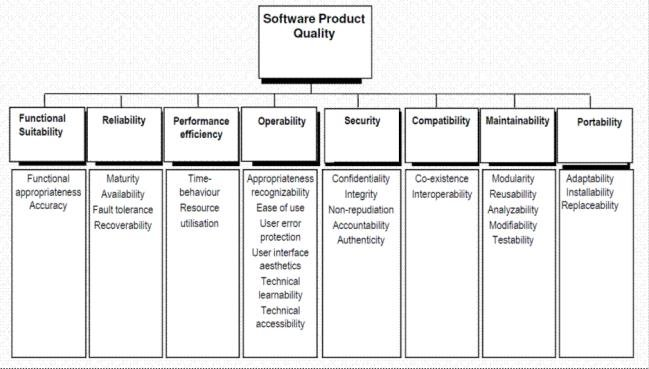
\includegraphics{images/ISO25010.jpg}\\*
\\*
\textbf{Παραπάνω παρουσιάζεται το ιεραρχικό μοντέλο: }
\textlatin{ISO25010}\\*

Η σημασία της ποιότητας του λογισμικού εξακολουθεί να αποτελεί βασικό ενδιαφέρον και για τα δύο
τις ακαδημαϊκές και βιομηχανικές κοινότητες μετά από περισσότερα από 50 χρόνια έρευνας
και πρακτική. Επιπλέον, όπως ο αριθμός των πολύπλοκων δικτυωμένων συστημάτων και
οι υποδομές ζωτικής σημασίας που στηρίζονται σε αυτές αυξάνονται, αναμένεται να παραμείνει α
θέμα συνεχούς ενδιαφέροντος για έρευνα, ανάπτυξη και συντήρηση λογισμικού.
Προηγούμενη έρευνα για την ποιότητα του λογισμικού είχε ως αποτέλεσμα μεγάλο αριθμό ποιότητας
μοντέλα. Τα περισσότερα από αυτά περιγράφουν ένα σύνολο βασικών ιδιοτήτων που προσπαθούν να το κάνουν
χαρακτηρίζουν τις πολλαπλές πτυχές ενός συστήματος λογισμικού από ένα εσωτερικό (προγραμματιστή-
προσανατολισμένη), εξωτερική (πελατοκεντρική) ή και των δύο προοπτικών.
Η εισαγωγή του πρώτου μοντέλου ποιότητας λογισμικού αποδίδεται στον \textlatin{McCall} in
1976, ακολουθούμενο από το μοντέλο \textlatin{Dromey} που το βελτίωσε. Αργότερα,
οι συνεισφορές έγιναν μέρος του προτύπου  \textlatin{ISO 9126}, το οποίο εξέφραζε λογισμικό
ποιότητας χρησιμοποιώντας ένα ιεραρχικό μοντέλο 5 τομέων ελέγχου που αποτελούνται από επιμέρους χαρακτηριστικά. Το μοντέλο  \textlatin{ISO 25010} που απεικονίζεται στο άνωθι σχήμα αντιπροσωπεύει την τρέχουσα έκδοση και θεωρεί τη δυνατότητα συντήρησης ως το σύνολο 5 βασικών
πυλώνων τροποποίησης: \\*
\begin{enumerate}
\item Αρθρωτότητα
\item Επαναχρησιμοποίηση
\item Αναλυσιμότητα
\item  Τροποποίηση
\item Δοκιμαστικότητα\\*
\end{enumerate}
\\*
Η ουσία αυτών των χαρακτηριστικών δεν είναι απαραίτητα να βελτιώνουν τον κώδικα ενός προγράμματος ή μια δομής προγραμμάτων (λογισμικού) αλλά να παράσχουν σχολαστικές λεπτομέρειες σχετικά με την δυνατότητα της περαιτέρω ανάπτυξης αυτού.\\*

Τα σημαντικά αποτελούμενα κομμάτια ενός λογισμικού εν γένει ονομάζονται \textlatin{metrics}.
Βασικές \textlatin{metrics} όπως γραμμές κώδικα, αριθμός συναρτήσεων ή αριθμός πακέτων και κλάσεων
οι ενότητες έχουν χρησιμοποιηθεί ευρέως και με τη σειρά τους, αντικαταστάθηκαν από την εισαγωγή του αντικειμενοστραφούς μοντέλου  και του σχετικού συνόλου μετρήσεων. Στις μέρες μας βρίσκουμε ένα
πλήθος αντικειμενοστρεφών \textlatin{metrics} όπως π.χ. αριθμός πακέτων και κλάσεων που ορίζονται και χρησιμοποιούνται για την ανίχνευση κομματιών κώδικα(προβληματικού),
ελαττωματικού σχεδιασμού ή για τη βελτίωση της συντηρησιμότητας. Αυτές οι μετρήσεις είναι επίσης
που απαιτούνται από τους ερευνητές για την αξιολόγηση της ποιότητας του λογισμικού σε ευρύτερο πλαίσιο. Ωστόσο, αυτό το μοντέλο φτάνει πια στην λήξη της λειτουργίας του στην αγορά και αντικαθίσταται πια από νέα που δίνουν έμφαση σε ποικίλους άλλους παράγοντες όπως η ταχύτητα του λογισμικού και η συμβασιμότητα αυτού με εργαλεία τεχνητης νοημοσύνης (ΑΙ) για την πιο υψηλού επιπέδου περάτωση και επίλυση ενός προβλήματος. 




















\subsection{Ταχύτητα}

% Costas
\subsection{Μοντέρνος Έλεγχος Ποιότητας}

Η παρακάτω ενότητα ασχολείται με τους σύγχρονους τρόπους ελέγχου της ποιότητας του λογισμικού. Ως επί το πλείστον, τα περισσότερα προγράμματα ανοιχτού κώδικα σχεδιάζονται και υλοποιούνται με την βοήθεια λογισμικού ελέγχου πηγαίου κώδικα(\textlatin{version control systems}), τα οποία επιτρέπουν σε μεγάλο αριθμό προγραμματιστών να συνεργάζονται πάνω στο ίδιο πρότζεκτ. Για αυτό το λόγο, η επόμενη υποενότητα αναλύει τα προγράμματα ελέγχου πηγαίου κώδικα.

\subsubsection{Λογισμικό Ελέγχου Πηγαίου Κώδικα}

Ο έλεγχος πηγαίου κώδικα ορίζεται ως η πρακτική σύμφωνα με την οποία παρακολουθούνται και διαχειρίζονται οι αλλαγές στον κώδικα του λογισμικού. Τα εργαλεία ελέγχου πηγαίου κώδικα είναι εξειδικευμένο λογισμικό, το οποίο συνεισφέρει στην διαχείριση του κώδικα από ομάδες προγραμματιστών. Ουσιαστικά, τα εν λόγω προγράμματα κρατούν κάθε αλλάγη στον πηγαίο κώδικα εντός μίας ειδικής βάσης δεδομένων. Εάν συμβεί κάποιο λάθος, οι προγραμματιστές μπορούν να επαναφέρουν τον πηγαίο κώδικα σε κάποια προηγούμενη έκδοση, αναιρώντας το πρόβλημα.

Επιπλέον, ο κώδικας ενός πρότζεκτ, μιας εφαρμογής ή ενός τμήματος λογισμικού είναι τυπικά οργανωμένος σε φακέλους. Έτσι, ένας προγραμματιστής μπορεί να δουλεύει ένα κομμάτι του κώδικας καθώς κάποιος άλλος αφαιρεί ένα \textlatin{bug} από ένα άλλο κομμάτι. Τα προγράμματα ελέγχου πηγαίου κώδικα συνεισφέρουν σε αυτή την διαδικασία καθώς καταγράφουν κάθε μεμονομένη αλλάγή από κάθε προγραμματιστή ξεχωριστά. Αλλαγές σε ένα κομμάτι του κώδικα ενδέχεται να μην είναι συμβατές με αυτές σε ένα άλλο τμήμα. Τέτοια προβλήματα πρέπει να αναγνωριστούν και να απομονωθούν δίχως να παρεμποδίζουν την ανάπτυξη του υπόλοιπου λογισμικού. Τα προγράμματα ελέγχου πηγαίου κώδικα μπορούν να διατηρούν πολλά κλαδιά(\textlatin{branches}) με διαφορετικές εκδόσεις του λογισμικού σε κάθε κλαδί, επιτρέποντας έτσι την εύκολη αντιμετώπιση των παραπάνω προβλημάτων.

Μακράν το πιο γνωστό λογισμικό ελέγχου πηγαίου κώδικα είναι το \textlatin{Git}. Το \textlatin{Git} είναι πλέον ενσωματωμένο σε πολλές πλατφόρμες και μπορεί να χρησιμοποιηθεί με πολλούς τρόπους. Γνωστά \textlatin{IDE} όπως το \textlatin{Visual Studio} της \textlatin{Microsoft}, το \textlatin{Android Studio} της \textlatin{Google} και πολλά άλλα, περιέχουν προεγκατεστημένο το \textlatin{Git} για πιο γρήγορο \textlatin{version control}. Υπάρχει φυσικά και η παραδοσιακή μέθοδος μέσω του \textlatin{terminal} ή και η επιλογή μίας γραφικής διεπαφής. Ακόμα, παρέχονται και διαδικτυές υπηρεσίες, όπως το \textlatin{Github}, το \textlatin{Gitlab} και το \textlatin{Bitbucket} που προσφέρουν γενικευμένες λύσεις στον τομέα του ελέγχου πηγαίου κώδικα. Άλλα λογισμικά ελέγχου πηγαίου κώδικα είναι το \textlatin{Mercurial} και το \textlatin{CVS(Concurrent Versions System)}.

\subsubsection{Αποφυγή Κακόβουλου Λογισμικού}

Το κύριο πρόβλημα ασφαλείας που αντιμετωπίζουν οι ομάδες ανάπτυξης ελεύθερου λογισμικού προκύπτει από το ότι ο καθένας είναι ελεύθερος να προσθέσει κώδικα στο πρότζεκτ. Κάποιος κακόβουλος προγραμματιστής θα μπορούσε να εισάγει λογισμικό το οποίο βλάπτει το πρόγραμμα ή τον χρήστη του. Για αυτό το λόγο, οι ομάδες που αναπτύσσουν τέτοιου είδους λογισμικό, σχεδόν πάντα, δεν επιτρέπουν την ενσωμάτωσει νέου κώδικα άνευ ελέγχου από κάποιο έμπειρο και έμπιστο μέλος της ομάδας. Ακόμα, ο νέος κώδικας συνηθίζεται να προστίθεται σε ξεχωριστά από το κεντρικό κλαδία του λογισμικού ελέγχου πηγαίου κώδικα. Έτσι, πριν την συγχώνευση των κλαδιών στο κεντρικό τμήμα, ο κώδικας επανελέγχεται για τυχόν επικίνδυνα κομμάτια κώδικα που διέφυγαν.

Ως αποτέλεσμα, ο λόγος για τον οποίο το λογισμικό ανοιχτού κώδικα θεωρείται και ασφαλείες είναι η ύπαρξη αυτής της "ομάδας ματιών" που συνεχώς κοιτάει τις νέες προσθήκες. Κάτι τέτοιο μπορεί να επιτευχθεί μόνο σε λογισμικό το οποίο είναι και διαθέσιμο άνευ πληρωμής, καθώς έτσι μπορεί να προσελκύσει μεγαλύτερο πλήθως ενδιφερομένων.

Παρόλα αυτά, πρέπει να σημειωθεί πως τα περισσότερα πρότζεκτ τα διαχειρίζονται μικρές, ολιγομελείς ομάδες. Έτσι, δεν είναι ιδιαίτερα απίθανη η διείσδυση κακόβουλου κώδικα στο λογισμικό, καθώς και ο αριθμός των ατόμων που τακτικά επιθεωρούν τις νέες προσθήκες είναι μικρότερος. Επιπλέον, εκ φύσεως το ανοιχτό λογισμικό δεν αναγκάζει τους συνδρομητές ενός πρότζεκτ να το συντηρήσουν. Οπότε, η δυνατότητα συντήρησης ενός πρότζεκτ μειώνεται καθώς οι προγραμματιστές που συνέσφεραν κώδικα φεύγουν και νέοι προγραμματιστές δεν είναι διατεθιμένοι να ανατρέξουν στον παλαιό κώδικα για να τον ανανεώσουν. Αυτό σημαίνει πως νέες αδυναμίες που ανακαλύπτονται με την πάροδο του χρόνου δεν διορθώνονται και το λογισμικό παραμένει επιρρεπής σε γνωστές πλέον επιθέσεις.

Κατά αυτό τον τρόπο έχουν υπάρξει ορισμένες περιπτώσεις όπου λογισμικό ανοιχτού κώδικα παρέμενε ευάλωτο σε επιθέσεις για πολλά χρόνια χωρίς αυτό να ήταν γνωστό στην ομάδα που το διαχειρίζοταν. Για παράδειγμα, στις 13
Μαΐου του 2008 ανακαλύφθηκε πως η έκδοση \textlatin{Debian} του λειτουργικού συστήματος \textlatin{Linux} διέθεται μία γεννήτρια τυχαίων αριθμών, της οποίας η συμπεριφορά μπορούσε να προβλεθεί. Αυτό έμπρακτα σήμαινε, πως χιλίαδες πακέτα είχα κρυπτογραφηθεί κατά τρόπο προβλέψιμο και έτσι η ακεραιότητα των εν λόγω πακέτων τέθηκε υπό αμφισβήτηση.

Άλλη μία γνωστή περίπτωση, όπου λογισμικού ανοιχτού κώδικα χτυπήθηκε και παρέμεινε μολυσμένο για μεγάλο χρονικό διάστημα είναι αυτή του \textlatin{Webmin}. Το \textlatin{Webmin} είναι λογισμικό διαχείρισης και ελέγχου διακομιστών τύπου \textlatin{Unix}. Ένας άγνωστος \textlatin{hacker} κατάφερε να εμφυτέψει ένα πρόγραμμα απομακρυσμένης πρόσβασης (\textlatin{backdoor}) εντός της επίσημης έκδοδης του \textlatin{Webmin}. Ως αποτέλεσμα, ο κακόβουλος χρήστης μπορούσε να αποκτήσει πρόσβαση σε κάθε υπολογιστή που κατέβαζε και εγκαταστούσε το \textlatin{Webmin}. Αργότερα, αναγνωρίστηκε από την ομάδα σύνταξης του προγράμματος πως η συγκεκριμένη αδυναμία είχε παραμείνει κρυμμένη για περισσότερο από ένα χρόνο.

\textbf{\section{Αναμενόμενα Αποτελέσματα}}







\section{Επίλογος}






\section{Βιβλιογραφία}
\textlatin{https://www.atlassian.com/git/tutorials/what-is-version-control}
\textlatin{https://www.debian.org/security/2008/dsa-1571}
}} %font
\end{document}